\documentclass[../differential_geometry.tex]{subfiles}
\begin{document}
\section{Aula 06 - de Fevereiro, 2026}
\subsection{Motivações}
\begin{itemize}
	\item Curvas em \(\mathbb{R}^{3}\);
	\item Triedro de Frenet;
	\item Curvatura;
	\item Torção;
	\item Teorema Fundamental de Curvas no Espaço;
	\item Forma Canônica.
\end{itemize}
\subsection{Curvas em no Espaço e o Teorema Fundamental de Curvas no Espaço}
Seja \(\alpha :I\rightarrow \mathbb{R}^{3}\) uma curva suave e regular parametrizada p.c.a; denotaremos por
\[
	t(s)=\frac{\mathrm{d}\alpha }{\mathrm{d}s}(s)=\alpha'(s)
\]
o vetor tangente unitário... Porém, não temos uma escolha canônica de uma rotação \(\pi/2\) do vetor \(t(s)\), e como ele é unitário,
\[
	\langle t, t \rangle = 1,
\]
onde emitimos o parâmetro s, e permanecerá assim a não ser que possa haver uma confusão. Logo,
\[
	\langle t', t \rangle=0,
\]
mostrando que \(t'\) é ortogonal a t.
\begin{figure}[H]
	\begin{center}
		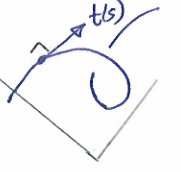
\includegraphics[height=0.4\textheight, width=0.4\textwidth, keepaspectratio]{./Images/tangent_vector_06.png}
	\end{center}
\end{figure}

\begin{def*}
	O \textbf{vetor normal a \(\mathbf{\alpha }\)} no ponto s é definido como o vetor
	\[
		n = \frac{1}{\Vert t' \Vert}t'. \; \square
	\]
\end{def*}
Como \(\kappa = \Vert t' \Vert\) por definição, vale também que \(t' = \kappa n\)
\begin{def*}
	O \textbf{vetor binormal à curva \(\mathbf{\alpha}\)} no ponto s é dado por
	\[
		b = t \times n,
	\]
	e o triedro \(\{t, n, b\}\) é chamado \textbf{triedro de Frenet}. \(\square\)
\end{def*}

O interesse no triedro de Frenet é que, para todo t, ele forma uma base ortonormal positiva de \(\mathbb{R}^{3}\) e se movimenta ao longo da curva \(\alpha \).
Vamos determinar as equações deste movimento: como \(\langle b, b \rangle=1\) e \(\langle b', b \rangle=0\), podemos derivar \(b=t \times n\) e obter
\[
	b'= t' \times n + t \times n',
\]
e como temos \(t'=\kappa n\), o termo \(t' \times n \) se anula (lembrando que \(n \times n=0\)). Daí,
\[
	\langle b', t \rangle = \langle t \times n', t \rangle=0.
\]
Logo,
\[
	\left.\begin{array}{ll}
		\langle b', b \rangle=0 \\
		\langle b', t \rangle=0
	\end{array}\right\} \Rightarrow b'\parallel n,
\]
e concluímos que, para algum escalar \(\tau (s)\),
\[
	b'(s)=\tau (s)n(s).
\]
\begin{def*}
	O escalar \(\tau (s)\) é chamado \textbf{torção da curva \(\mathbf{\alpha }\)} no ponto s. \(\square\)
\end{def*}

Com isso, o movimento do triedro de Frenet pode ser descrito como
\[
	n = b \times t = -t \times b,
\]
ou seja,
\[
	n'=-t'\times b-t \times b'=-\kappa n \times b-\tau t \times n.
\]
Portanto, o movimento do triedro de Frenet é descrito pela equações
\[
	\left\{\begin{array}{ll}
		t'=\kappa n           \\
		n'=-\kappa t - \tau b \\
		b'=\tau n
	\end{array}\right. \Longleftrightarrow \begin{pmatrix}
		t' \\
		n' \\
		b'
	\end{pmatrix} = \begin{pmatrix}
		0       & \kappa & 0     \\
		-\kappa & 0      & -\tau \\
		0       & \tau   & 0
	\end{pmatrix} \begin{pmatrix}
		t \\
		n \\
		b
	\end{pmatrix}.
\]

\begin{def*}
	O plano que passa pelo ponto \(\alpha (s)\) e que é gerado por \(t(s)\) e \(n(s)\) é chamado \textbf{plano osculador à curva \(\mathbf{\alpha} \)} no ponto s. \(\square\)
\end{def*}
\begin{def*}
	O plano que passa por \(\alpha (s)\) e que é gerado por \(n(s)\) e \(b(s)\) é chamado \textbf{plano normal à curva \(\mathbf{\alpha }\)} no ponto s. \(\square\)
\end{def*}
\begin{tcolorbox}[
		skin=enhanced,
		title=Observação,
		fonttitle=\bfseries,
		colframe=black,
		colbacktitle=cyan!75!white,
		colback=cyan!15,
		colbacklower=black,
		coltitle=black,
		drop fuzzy shadow,
		%drop large lifted shadow
	]
	Como \(b'=\tau n\), se a torção \(\tau (s)\) for nula em todo s do intervalo I, o vetor \(b(s)\) é constante, implicando à conclusão de que \(\alpha \) é uma curva plana. Logo, a torção mede a razão com a qual \(\alpha \) se afasta do plano osculador.
\end{tcolorbox}
\begin{exr}
	Prove a primeira parte da observação: como \(b'=\tau n\), se a torção \(\tau (s)\) for nula em todo s do intervalo I, o vetor \(b(s)\) é constante, implicando à conclusão de que \(\alpha \) é uma curva plana.
\end{exr}

\subsection{Calculando a curvatura e a torção}
Seja \(\alpha :I\rightarrow \mathbb{R}^{3}\), com u um parâmetro qualquer; denotaremos por s o parâmetro p.c.a., e temos
\[
	\frac{\mathrm{d}}{\mathrm{d}s} = \frac{1}{\Vert \alpha '(u) \Vert}\frac{\mathrm{d}}{\mathrm{d}u}.
\]
Podemos obter os valores de \(\kappa , \; n \;\&\; \tau \) pelos seguintes passos:
\begin{itemize}
	\item[1)] Calculamos \(\alpha '(u)\);
	\item[2)] Temos \(t(u)=\frac{\alpha '(u)}{\Vert \alpha '(u) \Vert}\);
	\item[3)] Obtemos \(\kappa \) e \(n\) por
	      \[
		      \frac{\mathrm{d}t}{\mathrm{d}s}=\frac{1}{\Vert \alpha '(u) \Vert}\frac{\mathrm{d}t}{\mathrm{d}u} = \kappa n;\;\&
	      \]
	\item[4)] Obtemos \(\tau \) com
	      \[
		      \frac{\mathrm{d}b}{\mathrm{d}s}=\frac{1}{\Vert \alpha '(u) \Vert}\frac{\mathrm{d}b}{\mathrm{d}u}=\tau n.
	      \]
\end{itemize}
De fato, pela igualdade em (3), segue que
\begin{align*}
	\frac{\mathrm{d}t}{\mathrm{d}s} = \frac{1}{\Vert \alpha '(u) \Vert}\frac{\mathrm{d}t}{\mathrm{d}u} & = \frac{1}{\Vert \alpha '(u) \Vert}\frac{\mathrm{d}}{\mathrm{d}u}\biggl(\frac{\alpha '(u)}{\Vert \alpha '(u) \Vert}\biggr)                                                              \\
	                                                                                                   & = \frac{1}{\Vert \alpha '(u) \Vert}\biggl[\frac{\alpha ''(u)}{\Vert \alpha '(u) \Vert} + \frac{\mathrm{d}}{\mathrm{d}u}\biggl(\frac{1}{\Vert \alpha '(u) \Vert}\biggr)\alpha'(u)\biggr] \\
	                                                                                                   & =\kappa n.
\end{align*}
Logo,
\begin{align*}
	 & ((\kappa n)\times t)(u)=\frac{1}{\Vert \alpha '(u) \Vert}\biggl[\frac{\alpha ''(u)}{\Vert \alpha '(u) \Vert} + \frac{\mathrm{d}}{\mathrm{d}u}\biggl(\frac{1}{\Vert \alpha '(u) \Vert}\biggr)\alpha '(u)\biggr] \times \frac{\alpha '(u)}{\Vert \alpha '(u) \Vert} \\
	 & (\kappa b)(u)= \frac{1}{\Vert \alpha '(u) \Vert^{3}}\alpha ''(n)\times \alpha '(u).
\end{align*}
Segue, portanto, que
\[
	\kappa (u)=\frac{\Vert \alpha ''(u)\times \alpha '(u) \Vert}{\Vert \alpha '(u) \Vert^{3}} = \frac{\Vert \alpha ''\times \alpha '\Vert}{\Vert \alpha '\Vert^{3}}
\]
\begin{exr}
	Mostre que
	\[
		\tau = - \frac{\langle \alpha ' \times \alpha '', \alpha ''' \rangle}{\Vert \alpha '\times \alpha '' \Vert^{2}}.
	\]
\end{exr}
\begin{example}
	A hélice é parametrizada por
	\[
		\alpha (u)=(a\cos^{}{u}, a \sin^{}{u}, bu),\quad u\in \mathbb{R},\; a>0,\; b\neq 0.
	\]
	Vamos calcular \(\kappa \) e \(\tau \).

	Para tanto, precisamos das 3 primeiras derivadas de \(\alpha \):
	\begin{align*}
		 & \alpha '=(-a \sin^{}{u}, a \cos^{}{u}, b)       \\
		 & \alpha '' = (-a \cos^{}{u}, -a \sin^{}{u}, 0)   \\
		 & \alpha ''' = (a \sin^{}{u}, - a \cos^{}{u}, 0).
	\end{align*}
	Disso, temos
	\begin{align*}
		 & \alpha ' \times \alpha '' = \det\begin{pmatrix}
			                                   \hat{i}       & \hat{j}       & \hat{k} \\
			                                   -a \sin^{}{u} & a \cos^{}{u}  & b       \\
			                                   -a \cos^{}{u} & -a \sin^{}{u} & 0
		                                   \end{pmatrix} = (ab \sin^{}{u}, -ab \cos^{}{u}, a^{2}) \\
		 & \Vert \alpha ' \times  \alpha '' \Vert = a \sqrt[]{a^{2}+b^{2}}                        \\
		 & \Vert \alpha ' \Vert = \sqrt[]{a^{2}+b^{2}},
	\end{align*}
	e concluímos que a curvatura é constante, valendo
	\[
		\kappa = \frac{a}{a^{2}+b^{2}}.
	\]
	Quanto à tração,
	\[
		\tau = - \frac{\langle \alpha ' \times \alpha '', \alpha '''  \rangle}{\Vert \alpha ' \times \alpha '' \Vert^{2}}=-\frac{a^{2}b}{a^{2}(a^{2}+b^{2})}=-\frac{b}{a^{2}+b^{2}},
	\]
	e concluímos que a torção também é constante:
	\[
		\tau = - \frac{b}{a^{2}+b^{2}}.
	\]
\end{example}

\begin{theorem*}
	Sejam \(\kappa (s)>0\) e \(\tau (s)\) duas funções suaves definidas em um intervalo aberto \(I\subseteq \mathbb{R}\); então, existe uma curva suave \(\alpha :I\rightarrow \mathbb{R}^{3}\) parametrizada p.c.a. tal que \(\kappa (s)\) e \(\tau (s)\) são a curvatura e a torção de \(\alpha.\) Além disso, a curva é única a menos de uma rotação e translação.
\end{theorem*}

\subsection{Forma Canônica}
Assim como fizemos para as curvas planas, podemos descrever uma base para a curva, descrevendo uma forma canônica para ela a partir de seu valor em um ponto! Sejam \(\alpha :I\rightarrow \mathbb{R}^{3} \) uma curva suave p.c.a., \(s_{0}\in I\) e
\[
	\Sigma = ({\color{DarkOrchid4}\alpha (s_{0})}, \{{\color{DarkOrange2}t(s_{0})}, {\color{Red3}n(s_{0})}, {\color{DarkGoldenrod2}b(s_{0}})\})
\]
um sistema de coordenadas em \(\mathbb{R}^{3}\). A partir disso, assim como antes, queremos obter uma expressão da curva no sistema de coordenadas \(\Sigma\), e podemos usar a fórmula de Taylor com \(s\in (s_{0}-\varepsilon , s_{0}+\varepsilon )\):
\[
	\alpha (s)={\color{DarkOrchid4}\alpha(s_{0})}+(s-s_{0}){\color{DarkOrange3}\alpha '(s_{0})}+\frac{(s-s_{0})^{2}}{2!}{\color{Red3}\alpha ''(s_{0})}+\frac{(s-s_{0})^{3}}{3!}{\color{DarkGoldenrod2}\alpha '''(s_{0})}+\mathcal{O}_{4}(s-s_{0}).
\]

Conforme a legenda de cores deixa indicado, em \(s_{0},\) temos
\begin{align*}
	 & {\color{DarkOrange3}\alpha '(s_{0})}={\color{DarkOrange3}t(s_{0})},                                                                                            \\
	 & {\color{Red3}\alpha ''(s_{0})}={\color{Red3}t'(s_{0})}={\color{Red3}\kappa (s_{0})n(s_{0})},                                                                   \\
	 & {\color{DarkGoldenrod2}\alpha'''(s_{0})}={\color{DarkGoldenrod2}\kappa '(s_{0})n(s_{0})+\kappa (s_{0})n'(s_{0})}                                               \\
	 & \quad\quad\quad  = {\color{DarkGoldenrod2}\kappa '(s_{0})n(s_{0})+\kappa (s_{0})(-\kappa(s_{0})t(s_{0})-\tau (s_{0})b(s_{0}))}                                 \\
	 & \quad\quad\quad = {\color{DarkGoldenrod2}-\kappa^{2}(s_{0})+\kappa '(s_{0})}{\color{Red3}n(s_{0})}-{\color{DarkGoldenrod2}\kappa (s_{0})\tau (s_{0})b(s_{0})}.
\end{align*}
Logo,
\begin{align*}
	\alpha (s)-{\color{DarkOrchid4}\alpha (s_{0})} & = (s-s_{0})t(s_{0}) + \frac{(s-s_{0})^{2}}{2!}\kappa (s_{0}){\color{Red3}n(s_{0})}+\frac{(s-s_{0})^{3}}{3!}({\color{DarkGoldenrod2}-\kappa^{2}(s_{0})+\kappa '(s_{0})}{\color{Red3}n(s_{0})} \\
	                                               & {-\color{DarkGoldenrod2}\kappa (s_{0})\tau (s_{0})b(s_{0})}) + \mathcal{O}_{4}(s-s_{0}).
\end{align*}
Assim, em coordenadas,
\begin{align*}
	\alpha (s)-{\color{DarkOrchid4}\alpha (s_{0})}  = \biggl( & {\color{DarkOrange3}s-s_{0}t(s_{0}) - \frac{\kappa^{2}(s_{0})}{3!}(s-s_{0})^{3}+\mathcal{O}_{4}(s-s_{0})},                \\
	                                                          & {\color{Red3}\frac{(s-s_{0})^{2}}{2!}\kappa (s_{0})+\frac{1}{3!}(s-s_{0})^{3}\kappa '(s_{0}) + \mathcal{O}_{4}(s-s_{0})}, \\
	                                                          & {\color{DarkGoldenrod2}-\frac{(s-s_{0})^{3}}{3!}\kappa (s_{0})\tau (s_{0})+ \mathcal{O}_{4}(s-s_{0})}\biggr).
\end{align*}
\begin{exr}
	Estude as projeções da curva \(\alpha \) no plano osculador e no plano normal.
\end{exr}

\end{document}

